\documentclass[1p]{elsarticle_modified}
%\bibliographystyle{elsarticle-num}

%\usepackage[colorlinks]{hyperref}
%\usepackage{abbrmath_seonhwa} %\Abb, \Ascr, \Acal ,\Abf, \Afrak
\usepackage{amsfonts}
\usepackage{amssymb}
\usepackage{amsmath}
\usepackage{amsthm}
\usepackage{scalefnt}
\usepackage{amsbsy}
\usepackage{kotex}
\usepackage{caption}
\usepackage{subfig}
\usepackage{color}
\usepackage{graphicx}
\usepackage{xcolor} %% white, black, red, green, blue, cyan, magenta, yellow
\usepackage{float}
\usepackage{setspace}
\usepackage{hyperref}

\usepackage{tikz}
\usetikzlibrary{arrows}

\usepackage{multirow}
\usepackage{array} % fixed length table
\usepackage{hhline}

%%%%%%%%%%%%%%%%%%%%%
\makeatletter
\renewcommand*\env@matrix[1][\arraystretch]{%
	\edef\arraystretch{#1}%
	\hskip -\arraycolsep
	\let\@ifnextchar\new@ifnextchar
	\array{*\c@MaxMatrixCols c}}
\makeatother %https://tex.stackexchange.com/questions/14071/how-can-i-increase-the-line-spacing-in-a-matrix
%%%%%%%%%%%%%%%

\usepackage[normalem]{ulem}

\newcommand{\msout}[1]{\ifmmode\text{\sout{\ensuremath{#1}}}\else\sout{#1}\fi}
%SOURCE: \msout is \stkout macro in https://tex.stackexchange.com/questions/20609/strikeout-in-math-mode

\newcommand{\cancel}[1]{
	\ifmmode
	{\color{red}\msout{#1}}
	\else
	{\color{red}\sout{#1}}
	\fi
}

\newcommand{\add}[1]{
	{\color{blue}\uwave{#1}}
}

\newcommand{\replace}[2]{
	\ifmmode
	{\color{red}\msout{#1}}{\color{blue}\uwave{#2}}
	\else
	{\color{red}\sout{#1}}{\color{blue}\uwave{#2}}
	\fi
}

\newcommand{\Sol}{\mathcal{S}} %segment
\newcommand{\D}{D} %diagram
\newcommand{\A}{\mathcal{A}} %arc


%%%%%%%%%%%%%%%%%%%%%%%%%%%%%5 test

\def\sl{\operatorname{\textup{SL}}(2,\Cbb)}
\def\psl{\operatorname{\textup{PSL}}(2,\Cbb)}
\def\quan{\mkern 1mu \triangleright \mkern 1mu}

\theoremstyle{definition}
\newtheorem{thm}{Theorem}[section]
\newtheorem{prop}[thm]{Proposition}
\newtheorem{lem}[thm]{Lemma}
\newtheorem{ques}[thm]{Question}
\newtheorem{cor}[thm]{Corollary}
\newtheorem{defn}[thm]{Definition}
\newtheorem{exam}[thm]{Example}
\newtheorem{rmk}[thm]{Remark}
\newtheorem{alg}[thm]{Algorithm}

\newcommand{\I}{\sqrt{-1}}
\begin{document}

%\begin{frontmatter}
%
%\title{Boundary parabolic representations of knots up to 8 crossings}
%
%%% Group authors per affiliation:
%\author{Yunhi Cho} 
%\address{Department of Mathematics, University of Seoul, Seoul, Korea}
%\ead{yhcho@uos.ac.kr}
%
%
%\author{Seonhwa Kim} %\fnref{s_kim}}
%\address{Center for Geometry and Physics, Institute for Basic Science, Pohang, 37673, Korea}
%\ead{ryeona17@ibs.re.kr}
%
%\author{Hyuk Kim}
%\address{Department of Mathematical Sciences, Seoul National University, Seoul 08826, Korea}
%\ead{hyukkim@snu.ac.kr}
%
%\author{Seokbeom Yoon}
%\address{Department of Mathematical Sciences, Seoul National University, Seoul, 08826,  Korea}
%\ead{sbyoon15@snu.ac.kr}
%
%\begin{abstract}
%We find all boundary parabolic representation of knots up to 8 crossings.
%
%\end{abstract}
%\begin{keyword}
%    \MSC[2010] 57M25 
%\end{keyword}
%
%\end{frontmatter}

%\linenumbers
%\tableofcontents
%
\newcommand\colored[1]{\textcolor{white}{\rule[-0.35ex]{0.8em}{1.4ex}}\kern-0.8em\color{red} #1}%
%\newcommand\colored[1]{\textcolor{white}{ #1}\kern-2.17ex	\textcolor{white}{ #1}\kern-1.81ex	\textcolor{white}{ #1}\kern-2.15ex\color{red}#1	}

{\Large $\underline{11a_{241}~(K11a_{241})}$}

\setlength{\tabcolsep}{10pt}
\renewcommand{\arraystretch}{1.6}
\vspace{1cm}\begin{tabular}{m{100pt}>{\centering\arraybackslash}m{274pt}}
\multirow{5}{120pt}{
	\centering
	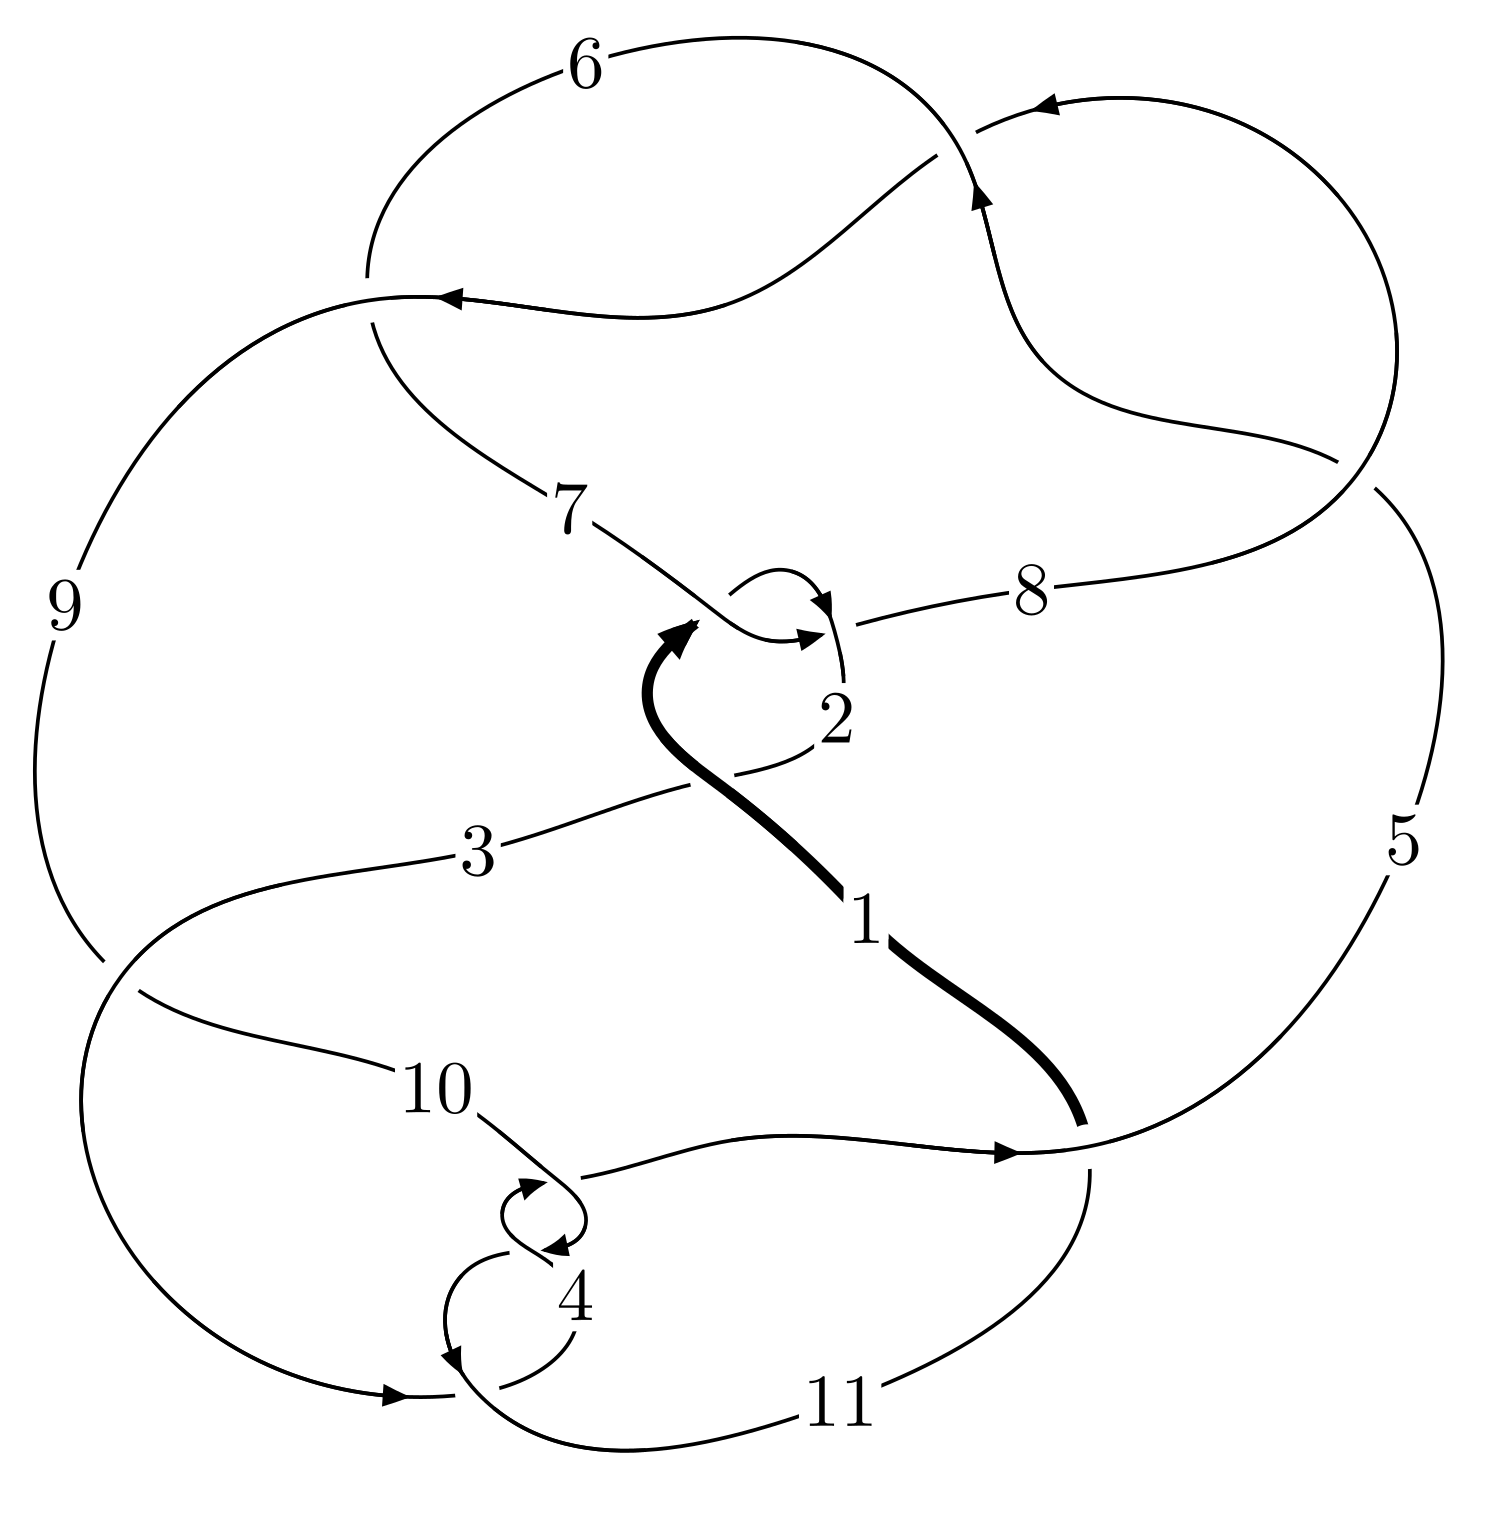
\includegraphics[width=112pt]{../../../GIT/diagram.site/Diagrams/png/490_11a_241.png}\\
\ \ \ A knot diagram\footnotemark}&
\allowdisplaybreaks
\textbf{Linearized knot diagam} \\
\cline{2-2}
 &
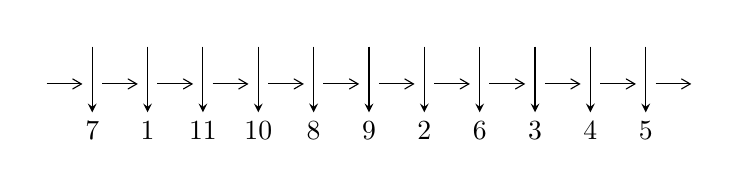
\begin{tikzpicture}[x=20pt, y=17pt]
	% nodes
	\node (C0) at (0, 0) {};
	\node (C1) at (1, 0) {};
	\node (C1U) at (1, +1) {};
	\node (C1D) at (1, -1) {7};

	\node (C2) at (2, 0) {};
	\node (C2U) at (2, +1) {};
	\node (C2D) at (2, -1) {1};

	\node (C3) at (3, 0) {};
	\node (C3U) at (3, +1) {};
	\node (C3D) at (3, -1) {11};

	\node (C4) at (4, 0) {};
	\node (C4U) at (4, +1) {};
	\node (C4D) at (4, -1) {10};

	\node (C5) at (5, 0) {};
	\node (C5U) at (5, +1) {};
	\node (C5D) at (5, -1) {8};

	\node (C6) at (6, 0) {};
	\node (C6U) at (6, +1) {};
	\node (C6D) at (6, -1) {9};

	\node (C7) at (7, 0) {};
	\node (C7U) at (7, +1) {};
	\node (C7D) at (7, -1) {2};

	\node (C8) at (8, 0) {};
	\node (C8U) at (8, +1) {};
	\node (C8D) at (8, -1) {6};

	\node (C9) at (9, 0) {};
	\node (C9U) at (9, +1) {};
	\node (C9D) at (9, -1) {3};

	\node (C10) at (10, 0) {};
	\node (C10U) at (10, +1) {};
	\node (C10D) at (10, -1) {4};

	\node (C11) at (11, 0) {};
	\node (C11U) at (11, +1) {};
	\node (C11D) at (11, -1) {5};
	\node (C12) at (12, 0) {};

	% arrows
	\draw[->,>={angle 60}]
	(C0) edge (C1) (C1) edge (C2) (C2) edge (C3) (C3) edge (C4) (C4) edge (C5) (C5) edge (C6) (C6) edge (C7) (C7) edge (C8) (C8) edge (C9) (C9) edge (C10) (C10) edge (C11) (C11) edge (C12) ;	\draw[->,>=stealth]
	(C1U) edge (C1D) (C2U) edge (C2D) (C3U) edge (C3D) (C4U) edge (C4D) (C5U) edge (C5D) (C6U) edge (C6D) (C7U) edge (C7D) (C8U) edge (C8D) (C9U) edge (C9D) (C10U) edge (C10D) (C11U) edge (C11D) ;
	\end{tikzpicture} \\
\hhline{~~} \\& 
\textbf{Solving Sequence} \\ \cline{2-2} 
 &
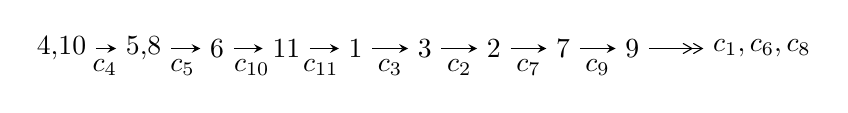
\begin{tikzpicture}[x=25pt, y=7pt]
	% node
	\node (A0) at (-1/8, 0) {4,10};
	\node (A1) at (17/16, 0) {5,8};
	\node (A2) at (17/8, 0) {6};
	\node (A3) at (25/8, 0) {11};
	\node (A4) at (33/8, 0) {1};
	\node (A5) at (41/8, 0) {3};
	\node (A6) at (49/8, 0) {2};
	\node (A7) at (57/8, 0) {7};
	\node (A8) at (65/8, 0) {9};
	\node (C1) at (1/2, -1) {$c_{4}$};
	\node (C2) at (13/8, -1) {$c_{5}$};
	\node (C3) at (21/8, -1) {$c_{10}$};
	\node (C4) at (29/8, -1) {$c_{11}$};
	\node (C5) at (37/8, -1) {$c_{3}$};
	\node (C6) at (45/8, -1) {$c_{2}$};
	\node (C7) at (53/8, -1) {$c_{7}$};
	\node (C8) at (61/8, -1) {$c_{9}$};
	\node (A9) at (10, 0) {$c_{1},c_{6},c_{8}$};

	% edge
	\draw[->,>=stealth]	
	(A0) edge (A1) (A1) edge (A2) (A2) edge (A3) (A3) edge (A4) (A4) edge (A5) (A5) edge (A6) (A6) edge (A7) (A7) edge (A8) ;
	\draw[->>,>={angle 60}]	
	(A8) edge (A9);
\end{tikzpicture} \\ 

\end{tabular} \\

\footnotetext{
The image of knot diagram is generated by the software ``\textbf{Draw programme}" developed by Andrew Bartholomew(\url{http://www.layer8.co.uk/maths/draw/index.htm\#Running-draw}), where we modified some parts for our purpose(\url{https://github.com/CATsTAILs/LinksPainter}).
}\phantom \\ \newline 
\centering \textbf{Ideals for irreducible components\footnotemark of $X_{\text{par}}$} 
 
\begin{align*}
I^u_{1}&=\langle 
u^{49}+2 u^{48}+\cdots+b-1,\;- u^{49}-2 u^{48}+\cdots+a+u,\;u^{50}+2 u^{49}+\cdots+2 u-1\rangle \\
I^u_{2}&=\langle 
b- u-1,\;u^2+a+u+2,\;u^3+u^2+2 u+1\rangle \\
\\
\end{align*}
\raggedright * 2 irreducible components of $\dim_{\mathbb{C}}=0$, with total 53 representations.\\
\footnotetext{All coefficients of polynomials are rational numbers. But the coefficients are sometimes approximated in decimal forms when there is not enough margin.}
\newpage
\renewcommand{\arraystretch}{1}
\centering \section*{I. $I^u_{1}= \langle u^{49}+2 u^{48}+\cdots+b-1,\;- u^{49}-2 u^{48}+\cdots+a+u,\;u^{50}+2 u^{49}+\cdots+2 u-1 \rangle$}
\flushleft \textbf{(i) Arc colorings}\\
\begin{tabular}{m{7pt} m{180pt} m{7pt} m{180pt} }
\flushright $a_{4}=$&$\begin{pmatrix}1\\0\end{pmatrix}$ \\
\flushright $a_{10}=$&$\begin{pmatrix}0\\u\end{pmatrix}$ \\
\flushright $a_{5}=$&$\begin{pmatrix}1\\u^2\end{pmatrix}$ \\
\flushright $a_{8}=$&$\begin{pmatrix}u^{49}+2 u^{48}+\cdots+9 u^2- u\\- u^{49}-2 u^{48}+\cdots- u+1\end{pmatrix}$ \\
\flushright $a_{6}=$&$\begin{pmatrix}u^{49}+2 u^{48}+\cdots+5 u^2+u\\- u^{48}-2 u^{47}+\cdots-2 u+1\end{pmatrix}$ \\
\flushright $a_{11}=$&$\begin{pmatrix}- u\\u\end{pmatrix}$ \\
\flushright $a_{1}=$&$\begin{pmatrix}- u^3-2 u\\- u^5- u^3+u\end{pmatrix}$ \\
\flushright $a_{3}=$&$\begin{pmatrix}u^2+1\\- u^2\end{pmatrix}$ \\
\flushright $a_{2}=$&$\begin{pmatrix}- u^{10}-5 u^8-8 u^6-3 u^4+3 u^2+1\\- u^{12}-4 u^{10}-4 u^8+2 u^6+3 u^4-2 u^2\end{pmatrix}$ \\
\flushright $a_{7}=$&$\begin{pmatrix}u^{49}+2 u^{48}+\cdots+5 u-1\\u^{49}+18 u^{47}+\cdots-2 u+1\end{pmatrix}$ \\
\flushright $a_{9}=$&$\begin{pmatrix}u^5+2 u^3+u\\- u^5- u^3+u\end{pmatrix}$\\ \flushright $a_{9}=$&$\begin{pmatrix}u^5+2 u^3+u\\- u^5- u^3+u\end{pmatrix}$\\&\end{tabular}
\flushleft \textbf{(ii) Obstruction class $= -1$}\\~\\
\flushleft \textbf{(iii) Cusp Shapes $= u^{49}+2 u^{48}+\cdots-5 u-13$}\\~\\
\newpage\renewcommand{\arraystretch}{1}
\flushleft \textbf{(iv) u-Polynomials at the component}\newline \\
\begin{tabular}{m{50pt}|m{274pt}}
Crossings & \hspace{64pt}u-Polynomials at each crossing \\
\hline $$\begin{aligned}c_{1},c_{7}\end{aligned}$$&$\begin{aligned}
&u^{50}+u^{49}+\cdots+20 u+8
\end{aligned}$\\
\hline $$\begin{aligned}c_{2}\end{aligned}$$&$\begin{aligned}
&u^{50}+21 u^{49}+\cdots+592 u+64
\end{aligned}$\\
\hline $$\begin{aligned}c_{3},c_{4},c_{10}\end{aligned}$$&$\begin{aligned}
&u^{50}-2 u^{49}+\cdots-2 u-1
\end{aligned}$\\
\hline $$\begin{aligned}c_{5},c_{6},c_{8}\end{aligned}$$&$\begin{aligned}
&u^{50}-4 u^{49}+\cdots-3 u-1
\end{aligned}$\\
\hline $$\begin{aligned}c_{9},c_{11}\end{aligned}$$&$\begin{aligned}
&u^{50}+2 u^{49}+\cdots-92 u-17
\end{aligned}$\\
\hline
\end{tabular}\\~\\
\newpage\renewcommand{\arraystretch}{1}
\flushleft \textbf{(v) Riley Polynomials at the component}\newline \\
\begin{tabular}{m{50pt}|m{274pt}}
Crossings & \hspace{64pt}Riley Polynomials at each crossing \\
\hline $$\begin{aligned}c_{1},c_{7}\end{aligned}$$&$\begin{aligned}
&y^{50}-21 y^{49}+\cdots-592 y+64
\end{aligned}$\\
\hline $$\begin{aligned}c_{2}\end{aligned}$$&$\begin{aligned}
&y^{50}+11 y^{49}+\cdots-19712 y+4096
\end{aligned}$\\
\hline $$\begin{aligned}c_{3},c_{4},c_{10}\end{aligned}$$&$\begin{aligned}
&y^{50}+42 y^{49}+\cdots-2 y+1
\end{aligned}$\\
\hline $$\begin{aligned}c_{5},c_{6},c_{8}\end{aligned}$$&$\begin{aligned}
&y^{50}-44 y^{49}+\cdots-3 y+1
\end{aligned}$\\
\hline $$\begin{aligned}c_{9},c_{11}\end{aligned}$$&$\begin{aligned}
&y^{50}-30 y^{49}+\cdots+70 y+289
\end{aligned}$\\
\hline
\end{tabular}\\~\\
\newpage\flushleft \textbf{(vi) Complex Volumes and Cusp Shapes}
$$\begin{array}{c|c|c}  
\text{Solutions to }I^u_{1}& \I (\text{vol} + \sqrt{-1}CS) & \text{Cusp shape}\\
 \hline 
\begin{aligned}
u &= -0.367759 + 1.080260 I \\
a &= \phantom{-}1.274030 - 0.076271 I \\
b &= -2.79298 - 1.22823 I\end{aligned}
 & -4.88671 - 5.18577 I & -14.7099 + 2.7132 I \\ \hline\begin{aligned}
u &= -0.367759 - 1.080260 I \\
a &= \phantom{-}1.274030 + 0.076271 I \\
b &= -2.79298 + 1.22823 I\end{aligned}
 & -4.88671 + 5.18577 I & -14.7099 - 2.7132 I \\ \hline\begin{aligned}
u &= -0.292411 + 1.122110 I \\
a &= \phantom{-}0.063602 + 0.178201 I \\
b &= \phantom{-}0.357273 + 0.494914 I\end{aligned}
 & \phantom{-}0.61352 - 1.42597 I & -11.17419 + 2.49743 I \\ \hline\begin{aligned}
u &= -0.292411 - 1.122110 I \\
a &= \phantom{-}0.063602 - 0.178201 I \\
b &= \phantom{-}0.357273 - 0.494914 I\end{aligned}
 & \phantom{-}0.61352 + 1.42597 I & -11.17419 - 2.49743 I \\ \hline\begin{aligned}
u &= -0.835547\phantom{ +0.000000I} \\
a &= \phantom{-}3.17253\phantom{ +0.000000I} \\
b &= \phantom{-}0.721481\phantom{ +0.000000I}\end{aligned}
 & -12.3381\phantom{ +0.000000I} & -20.6750\phantom{ +0.000000I} \\ \hline\begin{aligned}
u &= -0.815626 + 0.148361 I \\
a &= \phantom{-}2.61545 + 1.17715 I \\
b &= \phantom{-}0.549537 + 0.451977 I\end{aligned}
 & -7.73338 + 9.49487 I & -17.3734 - 6.5886 I \\ \hline\begin{aligned}
u &= -0.815626 - 0.148361 I \\
a &= \phantom{-}2.61545 - 1.17715 I \\
b &= \phantom{-}0.549537 - 0.451977 I\end{aligned}
 & -7.73338 - 9.49487 I & -17.3734 + 6.5886 I \\ \hline\begin{aligned}
u &= \phantom{-}0.304563 + 1.171450 I \\
a &= -2.12969 - 0.09359 I \\
b &= \phantom{-}4.12999 - 1.54851 I\end{aligned}
 & -2.05727 - 0.60926 I & -13.40155 + 0. I\phantom{ +0.000000I} \\ \hline\begin{aligned}
u &= \phantom{-}0.304563 - 1.171450 I \\
a &= -2.12969 + 0.09359 I \\
b &= \phantom{-}4.12999 + 1.54851 I\end{aligned}
 & -2.05727 + 0.60926 I & -13.40155 + 0. I\phantom{ +0.000000I} \\ \hline\begin{aligned}
u &= -0.777098 + 0.128997 I \\
a &= -0.922897 + 0.254550 I \\
b &= -0.222769 - 0.477721 I\end{aligned}
 & -2.36749 + 5.37835 I & -14.0557 - 6.0904 I\\
 \hline 
 \end{array}$$\newpage$$\begin{array}{c|c|c}  
\text{Solutions to }I^u_{1}& \I (\text{vol} + \sqrt{-1}CS) & \text{Cusp shape}\\
 \hline 
\begin{aligned}
u &= -0.777098 - 0.128997 I \\
a &= -0.922897 - 0.254550 I \\
b &= -0.222769 + 0.477721 I\end{aligned}
 & -2.36749 - 5.37835 I & -14.0557 + 6.0904 I \\ \hline\begin{aligned}
u &= \phantom{-}0.772297 + 0.099116 I \\
a &= -3.28933 + 1.31312 I \\
b &= -0.788912 + 0.473334 I\end{aligned}
 & -5.29863 - 3.31697 I & -16.7691 + 3.0814 I \\ \hline\begin{aligned}
u &= \phantom{-}0.772297 - 0.099116 I \\
a &= -3.28933 - 1.31312 I \\
b &= -0.788912 - 0.473334 I\end{aligned}
 & -5.29863 + 3.31697 I & -16.7691 - 3.0814 I \\ \hline\begin{aligned}
u &= -0.748495 + 0.067917 I \\
a &= -1.225140 - 0.393644 I \\
b &= \phantom{-}0.168459 + 0.395472 I\end{aligned}
 & -4.29681 + 0.76442 I & -18.3162 - 1.2723 I \\ \hline\begin{aligned}
u &= -0.748495 - 0.067917 I \\
a &= -1.225140 + 0.393644 I \\
b &= \phantom{-}0.168459 - 0.395472 I\end{aligned}
 & -4.29681 - 0.76442 I & -18.3162 + 1.2723 I \\ \hline\begin{aligned}
u &= -0.300001 + 1.216560 I \\
a &= -0.732766 - 0.843732 I \\
b &= \phantom{-}1.18393 + 1.18605 I\end{aligned}
 & -0.78921 + 3.02934 I & \phantom{-0.000000 } 0 \\ \hline\begin{aligned}
u &= -0.300001 - 1.216560 I \\
a &= -0.732766 + 0.843732 I \\
b &= \phantom{-}1.18393 - 1.18605 I\end{aligned}
 & -0.78921 - 3.02934 I & \phantom{-0.000000 } 0 \\ \hline\begin{aligned}
u &= \phantom{-}0.396406 + 0.624218 I \\
a &= \phantom{-}1.10662 - 1.27223 I \\
b &= -0.984367 + 0.603627 I\end{aligned}
 & -3.70738 - 5.14926 I & -14.3632 + 6.3732 I \\ \hline\begin{aligned}
u &= \phantom{-}0.396406 - 0.624218 I \\
a &= \phantom{-}1.10662 + 1.27223 I \\
b &= -0.984367 - 0.603627 I\end{aligned}
 & -3.70738 + 5.14926 I & -14.3632 - 6.3732 I \\ \hline\begin{aligned}
u &= \phantom{-}0.214240 + 1.257320 I \\
a &= \phantom{-}0.498732 + 0.074085 I \\
b &= -1.029970 + 0.417924 I\end{aligned}
 & \phantom{-}2.72213 - 2.30998 I & \phantom{-0.000000 } 0\\
 \hline 
 \end{array}$$\newpage$$\begin{array}{c|c|c}  
\text{Solutions to }I^u_{1}& \I (\text{vol} + \sqrt{-1}CS) & \text{Cusp shape}\\
 \hline 
\begin{aligned}
u &= \phantom{-}0.214240 - 1.257320 I \\
a &= \phantom{-}0.498732 - 0.074085 I \\
b &= -1.029970 - 0.417924 I\end{aligned}
 & \phantom{-}2.72213 + 2.30998 I & \phantom{-0.000000 } 0 \\ \hline\begin{aligned}
u &= \phantom{-}0.625043 + 0.306332 I \\
a &= \phantom{-}1.44268 - 0.83843 I \\
b &= -0.575863 + 0.474119 I\end{aligned}
 & -4.77278 + 1.48125 I & -17.3142 - 0.2721 I \\ \hline\begin{aligned}
u &= \phantom{-}0.625043 - 0.306332 I \\
a &= \phantom{-}1.44268 + 0.83843 I \\
b &= -0.575863 - 0.474119 I\end{aligned}
 & -4.77278 - 1.48125 I & -17.3142 + 0.2721 I \\ \hline\begin{aligned}
u &= -0.380094 + 1.257640 I \\
a &= \phantom{-}1.75256 + 1.12877 I \\
b &= -2.93137 - 3.26120 I\end{aligned}
 & -8.44132 + 4.36522 I & \phantom{-0.000000 } 0 \\ \hline\begin{aligned}
u &= -0.380094 - 1.257640 I \\
a &= \phantom{-}1.75256 - 1.12877 I \\
b &= -2.93137 + 3.26120 I\end{aligned}
 & -8.44132 - 4.36522 I & \phantom{-0.000000 } 0 \\ \hline\begin{aligned}
u &= \phantom{-}0.666165 + 0.120010 I \\
a &= \phantom{-}0.966211 + 0.119156 I \\
b &= \phantom{-}0.304071 - 0.280867 I\end{aligned}
 & -0.711738 - 0.697273 I & -10.71279 + 1.15101 I \\ \hline\begin{aligned}
u &= \phantom{-}0.666165 - 0.120010 I \\
a &= \phantom{-}0.966211 - 0.119156 I \\
b &= \phantom{-}0.304071 + 0.280867 I\end{aligned}
 & -0.711738 + 0.697273 I & -10.71279 - 1.15101 I \\ \hline\begin{aligned}
u &= -0.019632 + 1.351750 I \\
a &= \phantom{-}0.23638 - 1.46435 I \\
b &= \phantom{-}0.66874 + 2.33992 I\end{aligned}
 & \phantom{-}3.75475 + 1.24423 I & \phantom{-0.000000 } 0 \\ \hline\begin{aligned}
u &= -0.019632 - 1.351750 I \\
a &= \phantom{-}0.23638 + 1.46435 I \\
b &= \phantom{-}0.66874 - 2.33992 I\end{aligned}
 & \phantom{-}3.75475 - 1.24423 I & \phantom{-0.000000 } 0 \\ \hline\begin{aligned}
u &= -0.317517 + 1.315330 I \\
a &= \phantom{-}0.122364 - 0.368282 I \\
b &= \phantom{-}0.462053 + 0.996285 I\end{aligned}
 & \phantom{-}0.04307 + 4.61787 I & \phantom{-0.000000 } 0\\
 \hline 
 \end{array}$$\newpage$$\begin{array}{c|c|c}  
\text{Solutions to }I^u_{1}& \I (\text{vol} + \sqrt{-1}CS) & \text{Cusp shape}\\
 \hline 
\begin{aligned}
u &= -0.317517 - 1.315330 I \\
a &= \phantom{-}0.122364 + 0.368282 I \\
b &= \phantom{-}0.462053 - 0.996285 I\end{aligned}
 & \phantom{-}0.04307 - 4.61787 I & \phantom{-0.000000 } 0 \\ \hline\begin{aligned}
u &= \phantom{-}0.287032 + 1.337150 I \\
a &= \phantom{-}1.037980 - 0.647453 I \\
b &= -1.40488 + 1.30184 I\end{aligned}
 & \phantom{-}3.88325 - 4.20193 I & \phantom{-0.000000 } 0 \\ \hline\begin{aligned}
u &= \phantom{-}0.287032 - 1.337150 I \\
a &= \phantom{-}1.037980 + 0.647453 I \\
b &= -1.40488 - 1.30184 I\end{aligned}
 & \phantom{-}3.88325 + 4.20193 I & \phantom{-0.000000 } 0 \\ \hline\begin{aligned}
u &= \phantom{-}0.331579 + 1.330070 I \\
a &= -1.69831 + 2.26896 I \\
b &= \phantom{-}2.16421 - 5.01806 I\end{aligned}
 & -0.80897 - 7.30656 I & \phantom{-0.000000 } 0 \\ \hline\begin{aligned}
u &= \phantom{-}0.331579 - 1.330070 I \\
a &= -1.69831 - 2.26896 I \\
b &= \phantom{-}2.16421 + 5.01806 I\end{aligned}
 & -0.80897 + 7.30656 I & \phantom{-0.000000 } 0 \\ \hline\begin{aligned}
u &= \phantom{-}0.031726 + 1.385860 I \\
a &= \phantom{-}0.117801 + 1.234380 I \\
b &= -0.25515 - 1.61002 I\end{aligned}
 & \phantom{-}7.10349 - 2.64910 I & \phantom{-0.000000 } 0 \\ \hline\begin{aligned}
u &= \phantom{-}0.031726 - 1.385860 I \\
a &= \phantom{-}0.117801 - 1.234380 I \\
b &= -0.25515 + 1.61002 I\end{aligned}
 & \phantom{-}7.10349 + 2.64910 I & \phantom{-0.000000 } 0 \\ \hline\begin{aligned}
u &= -0.332926 + 1.345880 I \\
a &= -0.999826 - 0.769402 I \\
b &= \phantom{-}1.25204 + 1.35725 I\end{aligned}
 & \phantom{-}2.27588 + 9.39250 I & \phantom{-0.000000 } 0 \\ \hline\begin{aligned}
u &= -0.332926 - 1.345880 I \\
a &= -0.999826 + 0.769402 I \\
b &= \phantom{-}1.25204 - 1.35725 I\end{aligned}
 & \phantom{-}2.27588 - 9.39250 I & \phantom{-0.000000 } 0 \\ \hline\begin{aligned}
u &= \phantom{-}0.202172 + 0.562210 I \\
a &= -0.048043 + 0.695323 I \\
b &= \phantom{-}0.026647 + 0.413386 I\end{aligned}
 & \phantom{-}1.12881 - 2.03777 I & -7.78527 + 5.62795 I\\
 \hline 
 \end{array}$$\newpage$$\begin{array}{c|c|c}  
\text{Solutions to }I^u_{1}& \I (\text{vol} + \sqrt{-1}CS) & \text{Cusp shape}\\
 \hline 
\begin{aligned}
u &= \phantom{-}0.202172 - 0.562210 I \\
a &= -0.048043 - 0.695323 I \\
b &= \phantom{-}0.026647 - 0.413386 I\end{aligned}
 & \phantom{-}1.12881 + 2.03777 I & -7.78527 - 5.62795 I \\ \hline\begin{aligned}
u &= \phantom{-}0.237505 + 1.383800 I \\
a &= -0.179690 - 0.698918 I \\
b &= -0.46220 + 1.34014 I\end{aligned}
 & \phantom{-}0.55189 - 1.61966 I & \phantom{-0.000000 } 0 \\ \hline\begin{aligned}
u &= \phantom{-}0.237505 - 1.383800 I \\
a &= -0.179690 + 0.698918 I \\
b &= -0.46220 - 1.34014 I\end{aligned}
 & \phantom{-}0.55189 + 1.61966 I & \phantom{-0.000000 } 0 \\ \hline\begin{aligned}
u &= -0.350812 + 1.359940 I \\
a &= \phantom{-}1.22082 + 2.12971 I \\
b &= -1.48792 - 4.49301 I\end{aligned}
 & -2.97930 + 13.70140 I & \phantom{-0.000000 } 0 \\ \hline\begin{aligned}
u &= -0.350812 - 1.359940 I \\
a &= \phantom{-}1.22082 - 2.12971 I \\
b &= -1.48792 + 4.49301 I\end{aligned}
 & -2.97930 - 13.70140 I & \phantom{-0.000000 } 0 \\ \hline\begin{aligned}
u &= \phantom{-}0.06826 + 1.41694 I \\
a &= -0.365259 - 1.175510 I \\
b &= -0.35719 + 1.98198 I\end{aligned}
 & \phantom{-}2.73057 - 6.43368 I & \phantom{-0.000000 } 0 \\ \hline\begin{aligned}
u &= \phantom{-}0.06826 - 1.41694 I \\
a &= -0.365259 + 1.175510 I \\
b &= -0.35719 - 1.98198 I\end{aligned}
 & \phantom{-}2.73057 + 6.43368 I & \phantom{-0.000000 } 0 \\ \hline\begin{aligned}
u &= -0.166424 + 0.369815 I \\
a &= -1.27663 - 2.18999 I \\
b &= \phantom{-}1.009330 + 0.248240 I\end{aligned}
 & -1.55529 + 0.78493 I & -9.19094 - 1.36537 I \\ \hline\begin{aligned}
u &= -0.166424 - 0.369815 I \\
a &= -1.27663 + 2.18999 I \\
b &= \phantom{-}1.009330 - 0.248240 I\end{aligned}
 & -1.55529 - 0.78493 I & -9.19094 + 1.36537 I \\ \hline\begin{aligned}
u &= \phantom{-}0.299163\phantom{ +0.000000I} \\
a &= \phantom{-}0.652170\phantom{ +0.000000I} \\
b &= \phantom{-}0.313109\phantom{ +0.000000I}\end{aligned}
 & -0.616490\phantom{ +0.000000I} & -16.5510\phantom{ +0.000000I}\\
 \hline 
 \end{array}$$\newpage\newpage\renewcommand{\arraystretch}{1}
\centering \section*{II. $I^u_{2}= \langle b- u-1,\;u^2+a+u+2,\;u^3+u^2+2 u+1 \rangle$}
\flushleft \textbf{(i) Arc colorings}\\
\begin{tabular}{m{7pt} m{180pt} m{7pt} m{180pt} }
\flushright $a_{4}=$&$\begin{pmatrix}1\\0\end{pmatrix}$ \\
\flushright $a_{10}=$&$\begin{pmatrix}0\\u\end{pmatrix}$ \\
\flushright $a_{5}=$&$\begin{pmatrix}1\\u^2\end{pmatrix}$ \\
\flushright $a_{8}=$&$\begin{pmatrix}- u^2- u-2\\u+1\end{pmatrix}$ \\
\flushright $a_{6}=$&$\begin{pmatrix}- u^2- u-1\\u^2+u+1\end{pmatrix}$ \\
\flushright $a_{11}=$&$\begin{pmatrix}- u\\u\end{pmatrix}$ \\
\flushright $a_{1}=$&$\begin{pmatrix}u^2+1\\- u^2\end{pmatrix}$ \\
\flushright $a_{3}=$&$\begin{pmatrix}u^2+1\\- u^2\end{pmatrix}$ \\
\flushright $a_{2}=$&$\begin{pmatrix}u^2+1\\- u^2\end{pmatrix}$ \\
\flushright $a_{7}=$&$\begin{pmatrix}- u^2- u-2\\u+1\end{pmatrix}$ \\
\flushright $a_{9}=$&$\begin{pmatrix}-1\\- u^2\end{pmatrix}$\\ \flushright $a_{9}=$&$\begin{pmatrix}-1\\- u^2\end{pmatrix}$\\&\end{tabular}
\flushleft \textbf{(ii) Obstruction class $= 1$}\\~\\
\flushleft \textbf{(iii) Cusp Shapes $= -3 u^2-4 u-16$}\\~\\
\newpage\renewcommand{\arraystretch}{1}
\flushleft \textbf{(iv) u-Polynomials at the component}\newline \\
\begin{tabular}{m{50pt}|m{274pt}}
Crossings & \hspace{64pt}u-Polynomials at each crossing \\
\hline $$\begin{aligned}c_{1},c_{2},c_{7}\end{aligned}$$&$\begin{aligned}
&u^3
\end{aligned}$\\
\hline $$\begin{aligned}c_{3},c_{4}\end{aligned}$$&$\begin{aligned}
&u^3+u^2+2 u+1
\end{aligned}$\\
\hline $$\begin{aligned}c_{5},c_{6}\end{aligned}$$&$\begin{aligned}
&(u-1)^3
\end{aligned}$\\
\hline $$\begin{aligned}c_{8}\end{aligned}$$&$\begin{aligned}
&(u+1)^3
\end{aligned}$\\
\hline $$\begin{aligned}c_{9},c_{11}\end{aligned}$$&$\begin{aligned}
&u^3+u^2-1
\end{aligned}$\\
\hline $$\begin{aligned}c_{10}\end{aligned}$$&$\begin{aligned}
&u^3- u^2+2 u-1
\end{aligned}$\\
\hline
\end{tabular}\\~\\
\newpage\renewcommand{\arraystretch}{1}
\flushleft \textbf{(v) Riley Polynomials at the component}\newline \\
\begin{tabular}{m{50pt}|m{274pt}}
Crossings & \hspace{64pt}Riley Polynomials at each crossing \\
\hline $$\begin{aligned}c_{1},c_{2},c_{7}\end{aligned}$$&$\begin{aligned}
&y^3
\end{aligned}$\\
\hline $$\begin{aligned}c_{3},c_{4},c_{10}\end{aligned}$$&$\begin{aligned}
&y^3+3 y^2+2 y-1
\end{aligned}$\\
\hline $$\begin{aligned}c_{5},c_{6},c_{8}\end{aligned}$$&$\begin{aligned}
&(y-1)^3
\end{aligned}$\\
\hline $$\begin{aligned}c_{9},c_{11}\end{aligned}$$&$\begin{aligned}
&y^3- y^2+2 y-1
\end{aligned}$\\
\hline
\end{tabular}\\~\\
\newpage\flushleft \textbf{(vi) Complex Volumes and Cusp Shapes}
$$\begin{array}{c|c|c}  
\text{Solutions to }I^u_{2}& \I (\text{vol} + \sqrt{-1}CS) & \text{Cusp shape}\\
 \hline 
\begin{aligned}
u &= -0.215080 + 1.307140 I \\
a &= -0.122561 - 0.744862 I \\
b &= \phantom{-}0.78492 + 1.30714 I\end{aligned}
 & \phantom{-}1.37919 + 2.82812 I & -10.15260 - 3.54173 I \\ \hline\begin{aligned}
u &= -0.215080 - 1.307140 I \\
a &= -0.122561 + 0.744862 I \\
b &= \phantom{-}0.78492 - 1.30714 I\end{aligned}
 & \phantom{-}1.37919 - 2.82812 I & -10.15260 + 3.54173 I \\ \hline\begin{aligned}
u &= -0.569840\phantom{ +0.000000I} \\
a &= -1.75488\phantom{ +0.000000I} \\
b &= \phantom{-}0.430160\phantom{ +0.000000I}\end{aligned}
 & -2.75839\phantom{ +0.000000I} & -14.6950\phantom{ +0.000000I}\\
 \hline 
 \end{array}$$\newpage
\newpage\renewcommand{\arraystretch}{1}
\centering \section*{ III. u-Polynomials}
\begin{tabular}{m{50pt}|m{274pt}}
Crossings & \hspace{64pt}u-Polynomials at each crossing \\
\hline $$\begin{aligned}c_{1},c_{7}\end{aligned}$$&$\begin{aligned}
&u^3(u^{50}+u^{49}+\cdots+20 u+8)
\end{aligned}$\\
\hline $$\begin{aligned}c_{2}\end{aligned}$$&$\begin{aligned}
&u^3(u^{50}+21 u^{49}+\cdots+592 u+64)
\end{aligned}$\\
\hline $$\begin{aligned}c_{3},c_{4}\end{aligned}$$&$\begin{aligned}
&(u^3+u^2+2 u+1)(u^{50}-2 u^{49}+\cdots-2 u-1)
\end{aligned}$\\
\hline $$\begin{aligned}c_{5},c_{6}\end{aligned}$$&$\begin{aligned}
&((u-1)^3)(u^{50}-4 u^{49}+\cdots-3 u-1)
\end{aligned}$\\
\hline $$\begin{aligned}c_{8}\end{aligned}$$&$\begin{aligned}
&((u+1)^3)(u^{50}-4 u^{49}+\cdots-3 u-1)
\end{aligned}$\\
\hline $$\begin{aligned}c_{9},c_{11}\end{aligned}$$&$\begin{aligned}
&(u^3+u^2-1)(u^{50}+2 u^{49}+\cdots-92 u-17)
\end{aligned}$\\
\hline $$\begin{aligned}c_{10}\end{aligned}$$&$\begin{aligned}
&(u^3- u^2+2 u-1)(u^{50}-2 u^{49}+\cdots-2 u-1)
\end{aligned}$\\
\hline
\end{tabular}\newpage\renewcommand{\arraystretch}{1}
\centering \section*{ IV. Riley Polynomials}
\begin{tabular}{m{50pt}|m{274pt}}
Crossings & \hspace{64pt}Riley Polynomials at each crossing \\
\hline $$\begin{aligned}c_{1},c_{7}\end{aligned}$$&$\begin{aligned}
&y^3(y^{50}-21 y^{49}+\cdots-592 y+64)
\end{aligned}$\\
\hline $$\begin{aligned}c_{2}\end{aligned}$$&$\begin{aligned}
&y^3(y^{50}+11 y^{49}+\cdots-19712 y+4096)
\end{aligned}$\\
\hline $$\begin{aligned}c_{3},c_{4},c_{10}\end{aligned}$$&$\begin{aligned}
&(y^3+3 y^2+2 y-1)(y^{50}+42 y^{49}+\cdots-2 y+1)
\end{aligned}$\\
\hline $$\begin{aligned}c_{5},c_{6},c_{8}\end{aligned}$$&$\begin{aligned}
&((y-1)^3)(y^{50}-44 y^{49}+\cdots-3 y+1)
\end{aligned}$\\
\hline $$\begin{aligned}c_{9},c_{11}\end{aligned}$$&$\begin{aligned}
&(y^3- y^2+2 y-1)(y^{50}-30 y^{49}+\cdots+70 y+289)
\end{aligned}$\\
\hline
\end{tabular}
\vskip 2pc
\end{document}